\chapter{Realisation}


\section{Overview}

As explains above in the state of the art and in the figure\ref{tableau_comparatif} each approach has its advantages and its disadvantages. That is why in our solution we tried to take the better of the two worlds. We stylize the 3D scene in image space (screen space) but with all the information about the 3D object and the camera (camera matrices, position, normals, tangents, UV coordinates, distance from the camera). This solution permits to apply something like 2D images on the screen so have a good \textit{flatness} while keeping the information on the silhouettes, the orientation, the depth, etc. This solution permits also to easily integrate the stylizing of a scene in a pipeline rendering because it can be done at the end during the post-processing rendering pass. \newline

We chose to use mark based methods to stylize our scene because texture based methods in image space give a poor variety of styles as said in the work of Bénard et al.\cite{benard_dynamic_2009}. This mark based method implies to decide where in the image the splats will be drawn. In our problem, the goal is to anchor these splats with the objects in order to have the same motion for the splats and the object. This avoid the problem of \textit{shower door effect} and ensure the good \textit{motion coherence}. So we needed anchor points depending on the position of our object. Therefore in our approach, we used procedural noise\cite{perlin_improving_2002} as a texture of our 3D object. The procedural noises are easy to implement, fast to compute and easy to manipulate. Like every texture computed in object space, it has a good motion coherence. Each value different of zero of this texture represents an anchor point for a splat.


\section{Procedural noise and fractalization}

\begin{figure}
    \begin{center}
    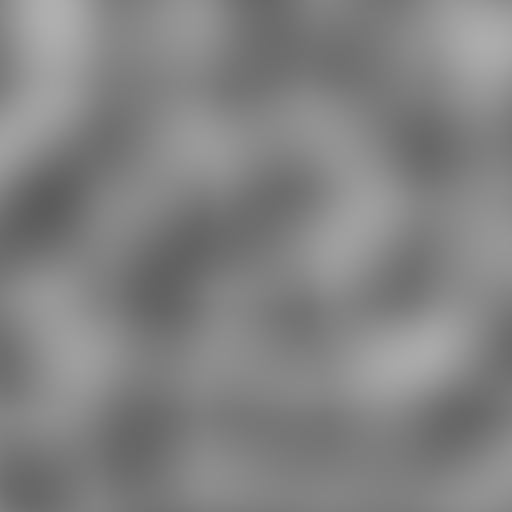
\includegraphics[width=40mm, height=40mm]{images/PerlinNoise2d.png}
    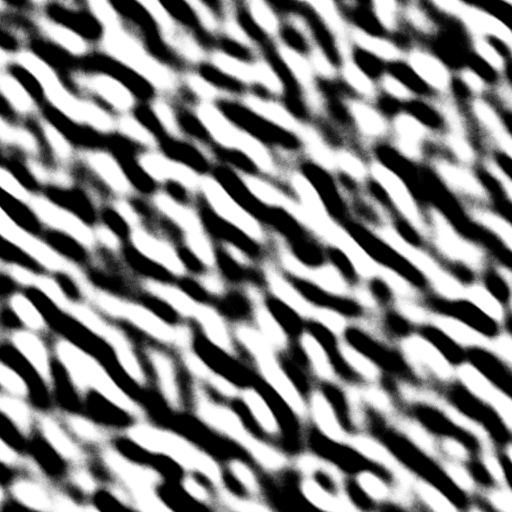
\includegraphics[width=40mm, height=40mm]{images/GaborNoise2d.png}
    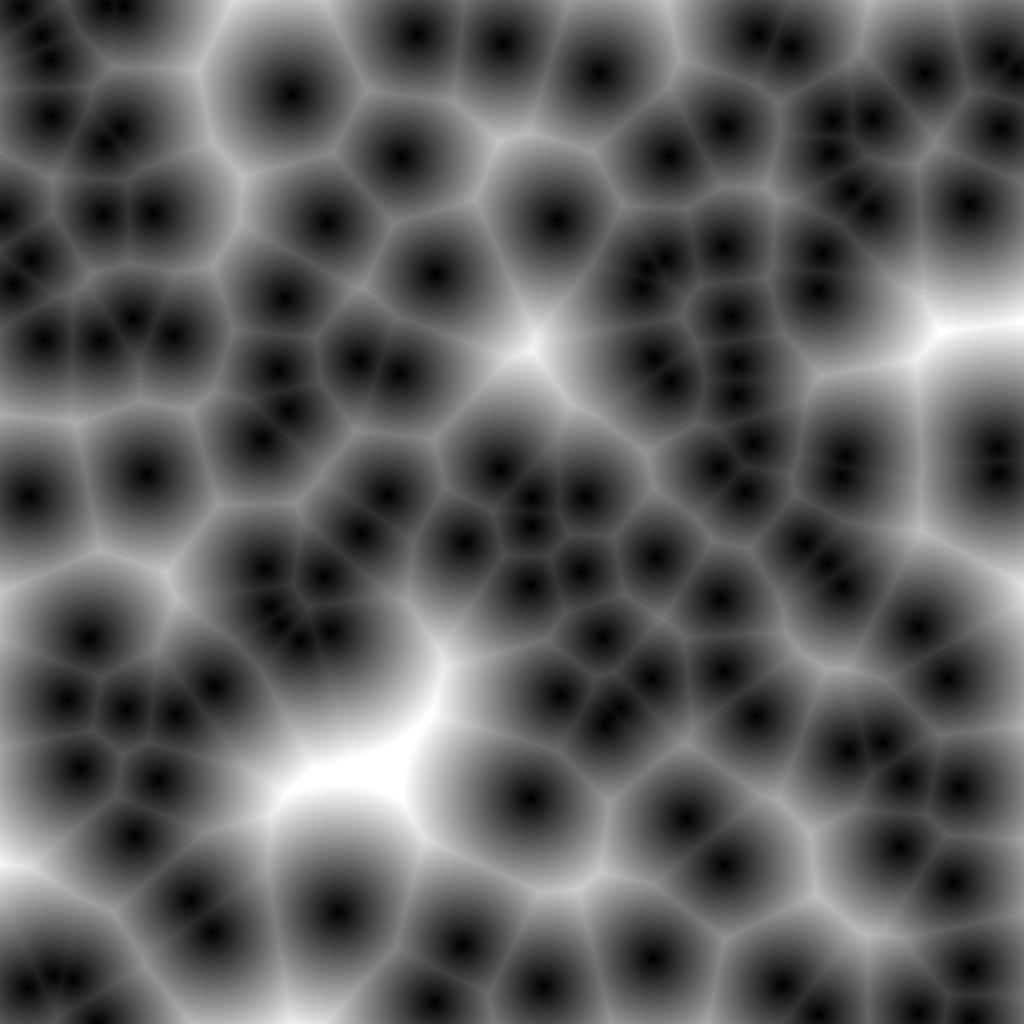
\includegraphics[width=40mm, height=40mm]{images/WorleyNoise2d.jpg}
    \end{center}
    \caption{Examples of procedural texture: \textit{left using perlin noise, middle using Gabor noise,right using worley noise}.}
    \label{procedural_texture}
\end{figure}

% Description of procedural noise

We compute procedural texture in order to create anchor points. Procedural noises are \textit{pseudorandom} gradient of grid point. In computer grapchis, they are usually used in 2d \ref{procedural_texture} as an image or in 3d for texturing a 3d object, in our case we use it in 3d. This texture are computed from procedural noise with a mathematical process. There exist many procedural noise such as Perlin noise, Worley noise, Gabor noise, Value noise, Gradient noise, etc. In order to map the procedural texture to the 3d object, we compute it with the vector position of each vertex of the object. The frequency of a noise control how many details there is in the texture. With a Worley noise, increasing the frequency will increase the number of black area in the texture.

% how we use it

\begin{figure}
    \begin{center}
    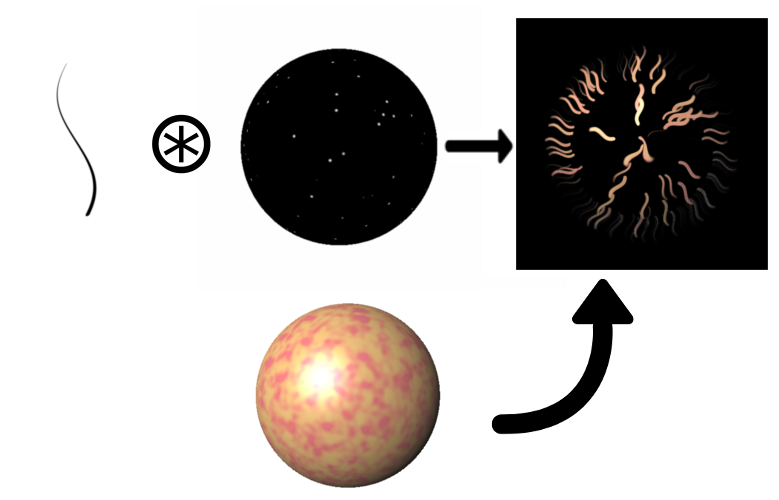
\includegraphics[scale=0.6]{images/noise/addition.png}
    \end{center}
    \caption{Usage of procedural texture to anchor splats: (left: splat image, middle: procedural teture, right: rendered image, bottom: color).}
    \label{procedural_noise_anchor}
\end{figure}

In our case we used the procedural texture to anchor the splat. For each pixel of the final image we "paste" a splat if the current pixel correspond to black pixel in the procedural texture the splat is not displayed (see Figure \ref{procedural_noise_anchor}). Thanks to this mechanism we can control the density of splat in the image. The value of our noise in the texture is between 0 and 1. The opacity vary according to this value of the procedural noise. One problem of working in image space is the aliasing, it creates some problem with \textit{temporal continuity} and \textit{motion coherence}. To reduce the aliasing in the procedural texture we make multiple samples with very small variation and we do an average to have the final value.

We add a threshold parameter to compute the noise in order to reduce the number of splat to display but especially to have small points in the procedural texture if not the splats convolve as you can see in the rendered image in the figure \ref{procedural_noise_anchor}.

% Worley

\begin{figure}
    \begin{center}
    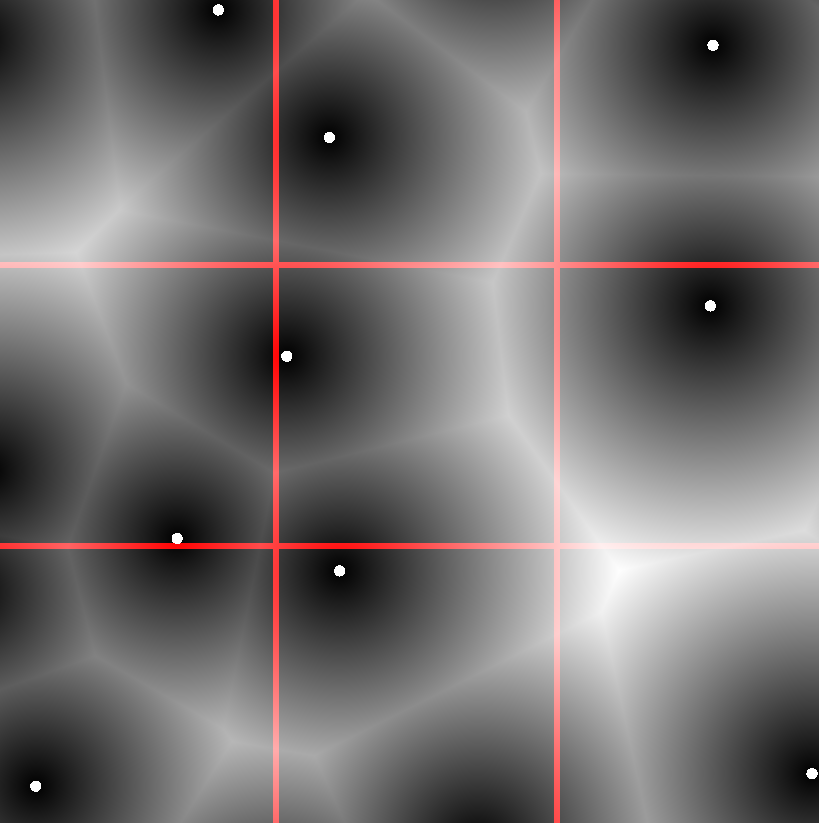
\includegraphics[scale=0.2]{images/noise/worley_explain.png}
    \end{center}
    \caption{Worley noise in 2d.}
    \label{worley_explain}
\end{figure}

We mainly work with the Worley noise which is a cellular noise as you can see at the right in the figure \ref{procedural_texture}. To create a procedural texture from a Worley noise, we divide the image in cells (squares with the same size in 2d and cubes with the same size in 3d, red lines in the figure \ref{worley_explain}), then in each square (cube in 3d) we compute a point with a seeded random (white dot in the figure \ref{worley_explain}) and finally at each pixel of the texture we put as value the distance with the closest point computed previously with the random seed. Increase the frequency of this noise correspond to divide the image with smaller cells and so have more cells in the image. In our pipeline we use the inverse of this noise (1-worleynoise) in order to have the white pixels of the procedural texture as anchor points.

\begin{figure}
    \begin{center}
    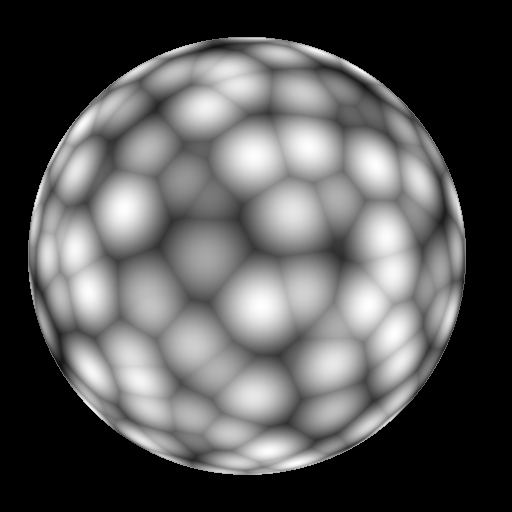
\includegraphics[scale=0.3]{images/noise/worley3d_thresh_1.png}
    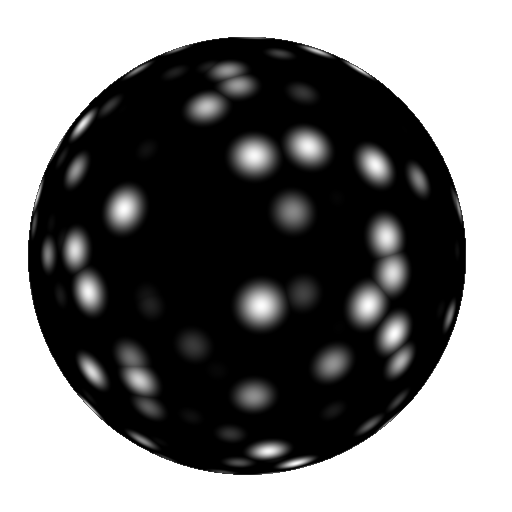
\includegraphics[scale=0.3]{images/noise/worley3d_thresh_2.png}
    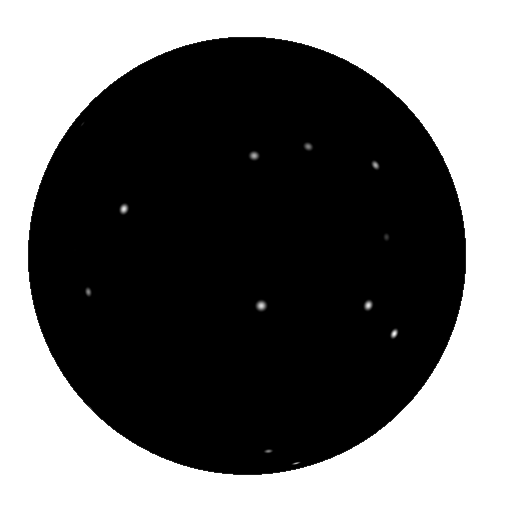
\includegraphics[scale=0.3]{images/noise/worley3d_thresh_3.png}
    \end{center}
    \caption{Use of threshold in the case of Worley noise with the same frequency.}
    \label{worley_threshold}
\end{figure}

As we said before we use a threshold for the purpose of having an another control on the noise. With the Worley noise this threshold correspond to the "size" of the points. If we increase the threshold the points become smaller as you can see in the figure \ref{worley_threshold}. In order to facilate the control of this noise we adapt this threshold according to frequency and the distance from the camera. That means that the size of each point is constant if the frequency or/and the distance from the camera is changed. \newline

% Add fractalization


\textbf{Fractalization}

\begin{figure}
    \begin{center}
    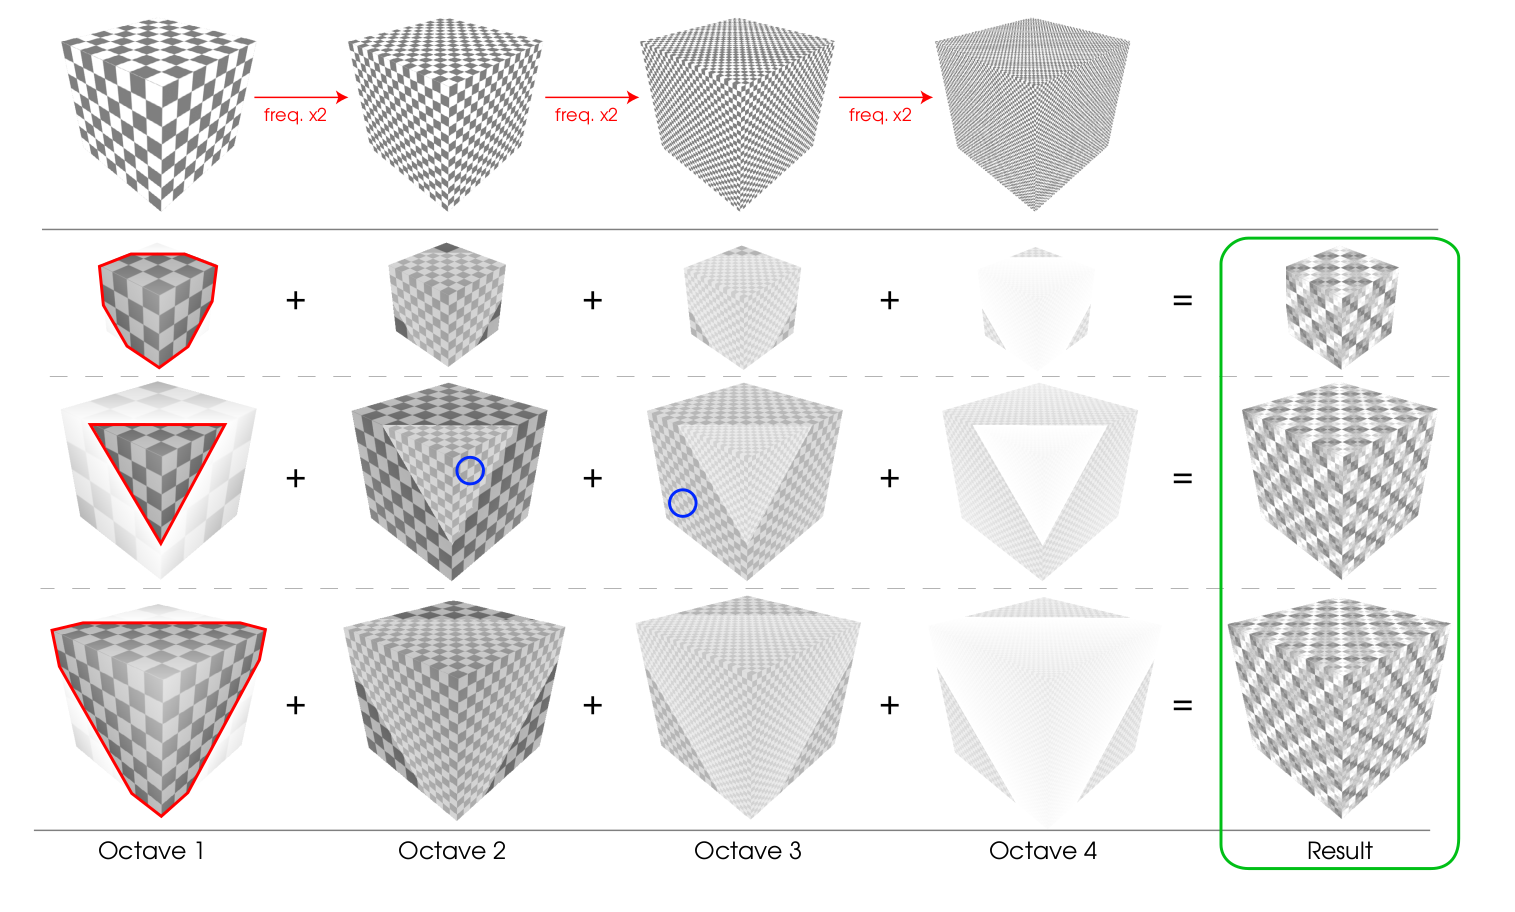
\includegraphics[scale=0.3]{images/fractalization_principle.png}
    \end{center}
    \caption{Principle of fractalization \cite{benard_dynamic_2010}.}
    \label{fractalization_principle}
\end{figure}

\begin{figure}
    \begin{center}
    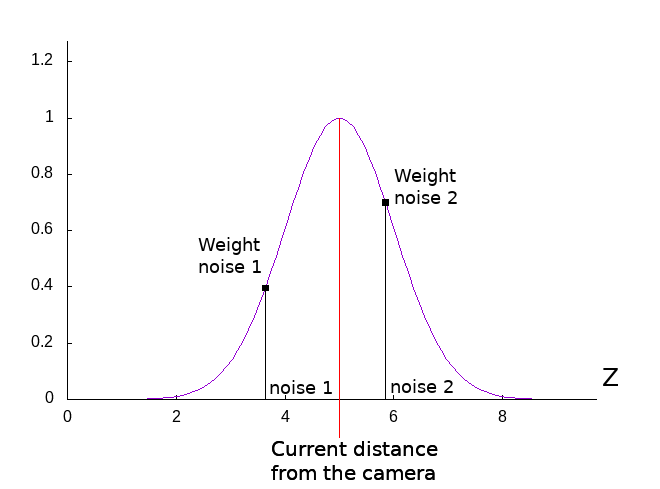
\includegraphics[scale=0.6]{images/fractal_explained.png}
    \end{center}
    \caption{Combination of the noises with the weight value in this case with 2 noises.}
    \label{fractalization_practical}
\end{figure}


Bénard et \textit{al.}\cite{benard_dynamic_2010} introduce the mechanism of fractalization on textures. This technique creates an impression of infinite zoom effect (like in this example: \href{https://www.shadertoy.com/view/XlBXWw?fbclid=IwAR1fU2JxQzXtks1ZcmVmzrHiv646G8w2gWceeiV-UToeFkAFMQ2NecbsGGs}{ShaderToy of Neyret Fabrice}). In our method of stylizing it improves the \textit{temporal continuity} because there is always display even if you get very close to the object and it also improves the \textit{flatness} impression because there is almost the same number of anchor points in the screen and their size is quasi-constant. This method alters the original pattern of the texture as you can see in the figure \ref{fractalization_principle} it can be an issue because some pattern cannot be fractalized (like the checkboard pattern) but it works well with stochastic textures. To creates this fractalization, they use textures at multiple frequencies (not necessary procedural texture) (see figure \ref{fractalization_principle}) and they combine them with the transparency and they overlap them according to the distance from the camera as you can see in the results of the figure \ref{fractalization_principle}. \newline


The figure \ref{fractalization_principle} show 4 noises (octaves) at different frequency it is a zooming cycle. As you can see, if the distance from the camera is close to 0 the frequency of the noises is high and if we move away from the object the frequency decrease. In the figure, we have: \texttt{2*frequency(octave 1) = frequency(octave 2)} and \texttt{2*frequency(octave 2) = frequency(octave 3)} and etc.  because in this case they divide the distance from the camera with a NON ! \textit{log2} so when the distance from camera is twice as large the frequency of the noise displayed is multiplied by 2. During the zoom, we modulate each octave with a weight. To compute the weight of each noise we use Gaussian interpolation centered on our current distance from the camera (see figure \ref{fractalization_practical}) with a sigma depending on the number of noises that we want to combine.







 % Bénard et \textit{al.}\cite{benard_dynamic_2010} use the same principle but with procedural textures. They create multiple noises with different frequency and combine them playing with transparency. Moreover, they overlap the noise to make an impression of infinite zoom effect (like in this example: \href{https://www.shadertoy.com/view/XlBXWw?fbclid=IwAR1fU2JxQzXtks1ZcmVmzrHiv646G8w2gWceeiV-UToeFkAFMQ2NecbsGGs}{ShaderToy}). With this method patterns of the texture have an almost constant size regardless of the size of the object but it can create small problems of \textit{temporal continuity}. In our method, we will use this technique of fractalization of a procedural noise. \newline

\section{Splatting}

\begin{figure}
    \begin{center}
    \fbox{
\includegraphics[width=30mm, height=30mm]{images/splats/dot_splat.png}}
    \fbox{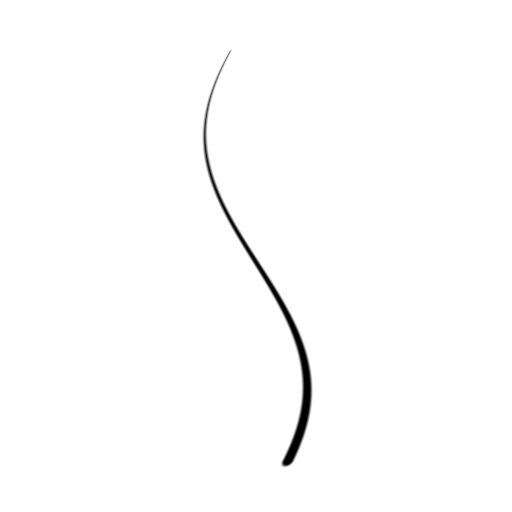
\includegraphics[width=30mm, height=30mm]{images/splats/hair_splat.png}}
    \fbox{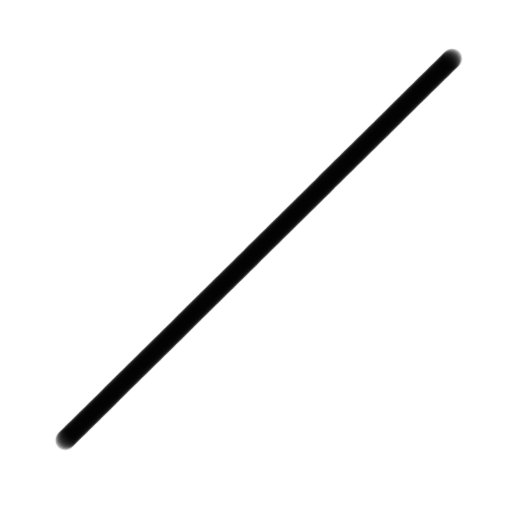
\includegraphics[width=30mm, height=30mm]{images/splats/line_splat.png}}
    \fbox{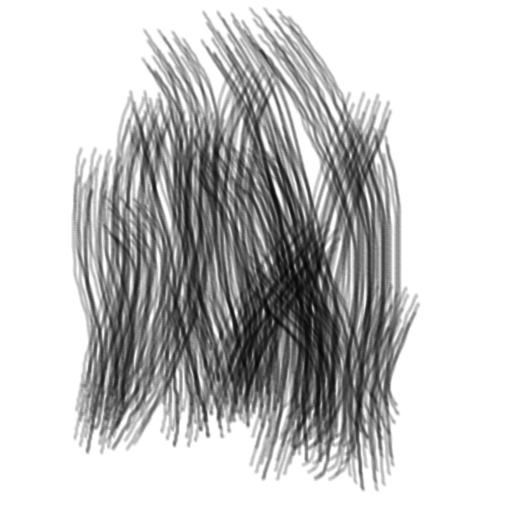
\includegraphics[width=30mm, height=30mm]{images/splats/paint_splat.png}}
    \end{center}
    \caption{Example of what the splats can be.}
    \label{splat_examples}
\end{figure}

The marks based method try to imitate how the artists do when they stylize. They draw on a flat surface that gives a good impression of \textit{flatness}. We use the same principle to stylize our scene. We put splats/marks directly on the image like an artist will do (illustrated in the figure \ref{procedural_noise_anchor}). \newline

In our solution, the user controls the splat image he can use anything. These marks can be leaves, hairs, dots, feathers, lines, paint brushes, etc. They can also be created from a procedural noise. The user has also the control on the size of these splats, he has a global control of the size and control on a specific part of the object through a texture. The rotation of the splats is also a parameter that the user can control. He can choose to rotate all the splat, for example, depending on the normals or depending on the tangents. \newline

Artists control how their marks are combined for example if he is doing painting he could want to have non-transparent marks in order to cover the marks behind the new one. He could want more transparency if for example he wants to do watercolorization.\newline

In our method, we take this into account during the blending of all marks. The user can control how many marks the stylization will mix and control the transparency (alpha blending). For example, the user can choose to only show the marks at the top of the flat surface (the closest to the camera) or he can choose to mix some marks in order to account some marks covered.


\section{Stylization}

As explained in the previous section, in our method, the user control the content of the splats, their size, their orientation, the density of splat on the object and how they are blended with the alpha blending. In this section, we will show you some examples of how we did specific style using our pipeline. \newline

\textbf{Pointillism}

\begin{figure}
    \begin{center}
    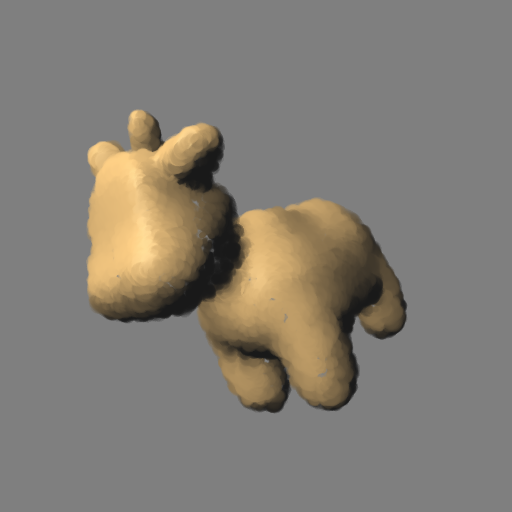
\includegraphics[width=80mm, height=80mm]{Resultats/spotPoint/final.png}
    \end{center}
    \caption{Example of pointillism with our method.}
    \label{final_point}
\end{figure}

In order to make pointillism style we use a dot as splat (gaussian fonction in 2d, the first in the figure \ref{splat_examples}), the procedural noise to control the number of splats has a high frequency, the size of the splats can vay depending on which size of brush he wants to imitate and for the alpha blending it usually adapt to not mix many marks. In this case the orientation does not matter. The figure \ref{final_point} shows the final rendered image.
